%\documentclass[twoside,openright,a4paper,11pt]{book}
%
%
\usepackage[utf8]{inputenc}
\usepackage[francais]{babel}
\usepackage[T1]{fontenc}

\addto\captionsfrench{\def\tablename{\textsc{Tableau}}}% pour avoir TABLEAU et pas TABLE dans les légendes des tableaux

%%%%%%% MISE EN PAGES %%%%%%
\usepackage{geometry}
\geometry{outer=2cm,inner=3cm,top=3cm}

\setcounter{tocdepth}{3}     % Dans la table des matieres
\setcounter{secnumdepth}{3}  % Avec un numero.
\usepackage{setspace}

\usepackage{fancyhdr}	% marge en haut et en bas
\pagestyle{fancy}

\fancyhead{}	% vide l'entête
\fancyfoot{} % vide le pied~de~page

\fancyhead[RO]{\leftmark}
\fancyhead[LE]{\rightmark}
\fancyfoot[C]{\thepage}	% numéro de page en bas au centre

\renewcommand{\headrulewidth}{0.4pt} % épaisseur du trait en haut
\renewcommand{\footrulewidth}{0.4pt} % épaisseur du trait en bas

\fancypagestyle{mypagestyle}{%
    \fancyhead{}	
    \fancyfoot{} 
    \fancyfoot[C]{\thepage}
    \renewcommand{\headrulewidth}{0.4pt} 
	\renewcommand{\footrulewidth}{0.4pt} 
}

\fancypagestyle{couvertureAbstract}{%
    \fancyhead{}	
    \fancyfoot{} 
    \fancyfoot[C]{}
	\renewcommand{\headrulewidth}{0pt} 
	\renewcommand{\footrulewidth}{0pt} 
}
%
\usepackage{layout}
\usepackage{tocbibind} % include tableofcontent in itself

%%%%%% PAGE DE GARDE %%%%%%

\geometry{outer=2cm,inner=3cm,top=3cm}
\usepackage[scaled]{helvet} % font used on cover (Helvetica)
\usepackage{eso-pic} % to set background picture
\usepackage{multicol} % for back cover (abstracts)
\usepackage{graphicx} % to include logos
\usepackage{tikz} % to compose background picture

% Colors (extracted from SPI's template)
\definecolor{boxcolor1}{rgb}{0.91373,0.92941,0.87451}
\definecolor{boxcolor2}{rgb}{0.94902,0.93333,0.91373}
\definecolor{boxcolor3}{rgb}{0.76078,0.87843,0.17647}
\definecolor{headercolor}{rgb}{0.94118,0.30980,0.17255}
\definecolor{namecolor}{rgb}{1.0,0.4,0.0}
\definecolor{titlecolor}{rgb}{0.19216,0.51765,0.60784}
% Also used: gray, teal (predefined by xcolor package, usually loaded by document class)

% Cover environment, to keep changes local
\newenvironment{cover}{%
  \fontfamily{phv}\selectfont % Select Helvetica font
  \pagestyle{empty} % No page number
}{
  \addtocounter{page}{-1}
  \cleardoublepage
}

% Macro for background common to front and back
\newcommand{\tikzBG}{%
  \path (0,0) rectangle (1,1);
  %TODO: You should adjust the bottom height of the following rectangle to fit your abstract's length
  \path [fill=boxcolor1] (.0571,.11) rectangle (.481,.963); 
  \path [fill=boxcolor2] (.4333,.697) rectangle (.9048,.7475);
  \path [fill=boxcolor2] (.4333,.7811) rectangle (.9048,.8316);
  \path [fill=boxcolor2] (.4333,.8687) rectangle (.9048,.9192);
  \path [fill=boxcolor3] (.0571,.7879) rectangle (.5762,.8316);
  \node[inner sep=0pt] at (0.2285,0.8788) [above left] {%
    
\includegraphics[height=.0707\paperheight,keepaspectratio]{./figures/logo/logo_unb.png}};
  \node[inner sep=0pt] at (0.6667,0.8788) [above right] {%
    
\includegraphics[height=.0808\paperheight,keepaspectratio]{./figures/logo/logo_ecn_color.png}};
  \node at (.0571,.8316) [above right,color=headercolor] {%
    \fontsize{29}{35}\selectfont\bfseries Th\`ese de Doctorat};
}

% Macro for repeated information (to avoid insconsistency)
%TODO: fill in with no formatting but desired case
\newcommand{\firstName}{Jean-Rémy}
\newcommand{\surname}{Gloaguen}
\newcommand{\thesisTitle}{Estimation du niveau sonore de sources d'intérêts au sein de mixtures sonores urbaines : application au trafic routier}

%%%%%%% SYMBOLES %%%%%
\usepackage{tipa}	% pour avoir l'accent concave
\usepackage{lmodern}	% pour les guillemets
\usepackage{gensymb}	% pour les degrés
\usepackage{enumitem}	% pour changer le symbole de l'item (\begin{itemize}[label=$\bullet$])

%%%%%%% EQUATION %%%%%%
\usepackage{amssymb}
\usepackage{amsmath}
\usepackage{fancybox}
\usepackage{xfrac}	% fraction de type "1/4"
\usepackage{cases}	% système équation
\usepackage[overload]{empheq}
\usepackage{bm}		% pour mettre en gras .
\usepackage{units} 	% x/y barre latérale pour les fractions
%
%%%%%%% FIGURE %%%%%%
\usepackage{subfigure}	% utiliser subfigure
\usepackage{float}	% utiliser H dans les figures
%
%%%%%% TABLEAUX %%%%%%
\usepackage{array,multirow,makecell}
%\addto\captionsfrench{\def\tablename{\textsc{Tableau}}}% pour avoir TABLEAU et pas TABLE dans les légendes des tableaux
\usepackage{colortbl} % pour avoir des lignes colorées dans les tableau
%\usepackage{slashbox} % pour les \backslashbox
%\usepackage{subcaption}
\usepackage{hhline}	% pour les lignes horizontales 
\usepackage{tabularx} % permet itemize dans les cellules
\usepackage{booktabs}
\usepackage{longtable}	% pour les tableaux longs

\newcolumntype{L}[1]{>{\raggedright\let\newline\\\arraybackslash\hspace{0pt}}m{#1}}
\newcolumntype{C}[1]{>{\centering\let\newline\\\arraybackslash\hspace{0pt}}m{#1}}
\newcolumntype{R}[1]{>{\raggedleft\let\newline\\\arraybackslash\hspace{0pt}}m{#1}}

%%%%% ALGORITHME %%%%%
\usepackage{algorithm}
\usepackage{algorithmic}

%%%%% BIBLIO %%%%%
\usepackage[fixlanguage]{babelbib}
\selectbiblanguage{french}
\usepackage{breakcites}	% pour couper les références en bout de ligne

%%%%% APPENDICES %%%%%%%
\usepackage[toc,page]{appendix}

%%%%%%%%%%%%%%%%%%%%%
\usepackage{url}	% gérer les adresses www.
\linespread{1.2}	% interligne

\cleardoublepage
%
%\begin{document}
%\newpage

\chapter{Identification, détection et séparation des sources sonores}

La détection, l'identification ou la séparation d'une source sonore dans le cadre de sons environnementaux (qui ne contiennent ni de la musique, ni de la parole) est un sujet complexe car cette catégorie inclut des sons extrêmement variés aussi bien en temps qu'en fréquence. De prime abord, ces méthodes de traitement du signal ont été appliquées pour des signaux contenant de la voix et de la musique car leur structure est beaucoup mieux prédictive et connue. L'application de ces méthodes se fait en deux phases : une phase d'apprentissage où les algorithmes sont testé sur des bases de données connues et qui permet de déterminer le comportement de l'outil puis une phase de test où ce modèle est appliqué à une base de données inconnues. De nombreuses études se sont intéressés à savoir détecter les différents évènements sonores présent dans un scène. Les outils utilisés seront présenté dans la partie \ref{sec:ident_detec}. Enfin, souhaitant isoler le trafic routier des autres sources sonores, ce sont les méthodes de séparation de sources qui seront revues dans la partie

\section{Méthodes de détection et d'identification}
\label{sec:ident_detec}

Lorsqu'on parle de classification, il s'agit de savoir automatiquement savoir si un extrait audio appartient à une catégorie ou à une autre. Il peut s'agir de classer un morceau de musique selon son style \cite{tzanetakis_musical_2002}, de classer un enregistrement sonore selon son environnement sonore \cite{chu_where_2006}. Lorsqu'on parle de détection, on parle de la détermination du temps de présence des différents évènements sonores dans un scène sonore mais également à déterminer la source sonore correspondante. Cette tâche trouve notamment son intérêt lors des phases d'annotation de scènes sonore où un auditeur estime à la main le temps d'apparition et de fin des différents évènements, tâche qui peut être très fastidieuse et complexe \cite{mesaros_sound_2015} \cite{cakir_polyphonic_2015}. \\

Afin de comparer les performances des algorithmes, plusieurs bases de données on été conçu, lors de challenges, afin d'être utiliser pour les tester. Dans le cas de la parole, la base de données CHiME \cite{christensen_chime_2010} est la plus souvent utilisée \cite{barker_pascal_2013} \cite{araki_2011_2012}. Pour la musique, des bases de données, comme RWC \cite{goto_rwc_2003} et CAL500 \cite{wang_towards_2014}, existent et servent pour des tâches comme la classification par genre musicaux ou à la définition des structures musicales. Certaines base de données sont même destinées à une classe d'instrument particulière (comme les instruments percussifs pour la base de données , ENST-drums \cite{gillet_enst-drums:_2006}). \\

Si ces base de données et challenge on été destiné à la parole et à la musique, c'est à partir de 2013 qu'est crée le challenge \textit{Detection $\&$ Classification of Acoustics Scene Event} (DCASE) \cite{giannoulis_detection_2013} qui s'adresse aux sons environnementaux. La lecture des articles résumant les techniques ainsi que les résultats permet de connaitre les méthodes qui sont plébiscités. \\


De nombreux modèles de classificateur ou de détecteur adapté à des sons urbains utilisent les même outils que pour les sons de paroles ou musicaux. Cette partie présente les approches et les différents outils les plus couramment utilisés. Le modèle de classification est réalisée en deux étapes. Les signaux audio sont d'abord décrits par des descripteurs qui vont donner une représentation réduite des classes de sons visées. Un classificateur est ensuite utilisé permettant ainsi de distinguer les différentes classes de sons présentes dans le signal audio. La partie~\ref{part:descripteur} et \ref{part:classificateur} exposent respectivement les différents descripteurs et classificateurs couramment utilisées.

\subsection{Descripteurs}\label{part:descripteur}
Un large nombre de descripteurs ont déjà été utilisé dans la littérature \cite{} \cite{} \cite{}. Ces descripteurs peuvent décrire un signal à la foi dans le domaine temporel que fréquentiel. Ils permettent de réduire la dimension du signal audio à quelques valeurs simplifiant la classification. Pour être optimal, le choix de ces descripteurs doit permettre une description unique des classes de sons. Dans \cite{}, Peeters résume un grand nombre de paramètres couramment utilisé qu'il regroupe dans le projet CUIDADO. Il classe les paramètres en 5 familles : les paramètres temporels, énergétiques, spectraux, harmoniques et perceptifs.

\begin{itemize}
\item \textbf{paramètres temporels} : il résume aussi bien les paramètres qui décrive un signal sur des parties entière du signal (par exemple l'attaque, la tenue et l'extinction du isgnal) que de manière instantanée avec la fonction d'auto-corrélation ou le \textit{Zero-Crossing Rate} qui énumère le nombre de fois qu'un signal traverse l'axe des zéro. Un faible ZCR traduit un signal harmonique alors qu'un grand ZCR signifie le son est composé de bruit. 

\item \textbf{paramètres énergétiques} : Il résume les indicateurs énergétique aussi bien du signal entier que de partie plus restreinte ou bien encore celles des composantes harmoniques ou du bruits.

\item \textbf{paramètres spectrales} : C'est une classe de descripteurs large. Elle contient des descripteurs simples comme le centre de gravité spectrale ou qui calcule l'évolution temporel du spectre (ou flux spectral) comme des descripteurs plus complexe comme les LPCC (Linear Predictive Cepstral Coefficient) et les MFCC (Mel Frequency Cepstral Coefficient). Les MFCC sont couramment utilisés dans les tâches de classification ou de détection. Ils consistent à exprimer la transformée de Fourier d'un signal par des bandes Mel et à réaliser à transformée en cosinus discret du logarithme du signal obtenu (figure \ref{fig:schema_mfcc}).

\begin{figure}[h]
\centering
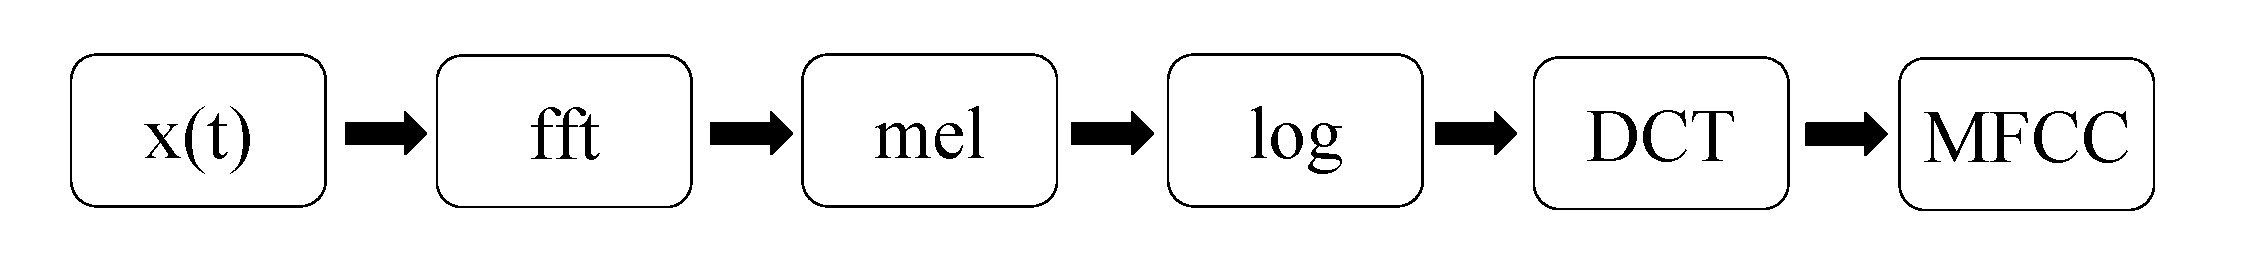
\includegraphics[width = 0.7\textwidth]{./figures/autres/schema_MFCC.pdf}
\caption{Schéma de la conception des MFCC}
\label{fig:schema_mfcc}
\end{figure}

L'échelle Mel est une échelle de hauteur de sons issus de la psycho-acoustique. Son échelle est construite afin qu'un doublement de mel corresponde à un doublement de la fréquence perçu. Par exemple pour un son pur à 1000 Hz (correspondant à 1000 mel), le son perçu deux fois plus aigu sera un son à environ 3428 Hz et non à 2000 Hz. L'échelle des Mel est alors définit par la relation \ref{eq:melScale} permettant ainsi de conserver le rapport 2 entre les deux sons (le signal à 3428 Hz est alors à 2000 mel),

\begin{equation}\label{eq:melScale}
mel = 1127 \ln\left(1+\frac{f}{700}\right).
\end{equation}


\item \textbf{paramètres harmoniques} : Cette catégorie regroupe des descripteurs comme la détermination de la fréquence fondamental, de  l'inharmonicité ou bien du tristimulus du signal.

\item \textbf{paramètres perceptifs} : Cette dernière classe regroupe les indicateurs psycho-acoustique comme l'acuité ou la sonie du signal.\\
\end{itemize}

Dans son article, Peeters \cite{Peeters} résume un ensemble de descripteurs couramment utilisés dans le domaine de la reconnaissance de parole \cite{Kim} ou le domaine de la musique \cite{Fu} qui sont ceux qui sont également utilisés pour des ambiances sonores environnementales \cite{Cowling}, \cite{Haddad}, \cite{Defreville}. 


%
%En raison de l'utilisation de l'échelle Mel, les MFCC sont le plus souvent utilisés dans le cas de la détection de signaux de paroles \cite{Wu}.

%\subsection{Analyse en Composante Principale}\label{part:ACP}
%
%L'utilisation de plusieurs descripteurs génèrent un ensemble de données décrivant chaque signal spécifiquement. 
%
%\begin{equation}
%\mathbf{X} = 
%\begin{pmatrix}
%x_{11}& x_{12} & \dots & x_{1p} \\
%x_{21}& x_{22} & \dots & x_{2p} \\
%\vdots & \vdots & \ddots & \vdots \\
%x_{N1}& x_{N2} & \dots & x_{Np}
%\end{pmatrix}
%\end{equation}
%
%où $N$ est le nombre de signaux traités et $p$ le nombre de variable utilisé pour les décrire. Néanmoins, leur représentation graphique en un nuage de point qui permettrait de visualiser la corrélation entre les signaux n'est pas facile au delà de $p = 3$ car la dimension de problème n'est alors plus représentable. De plus, certains paramètres sont parfois redondant et ajoute une dimension aux problème rendant la représentations des corrélations entre elles plus difficile. \\
%
%L'Analyse en Composante Principale (ACP) se propose alors de réduire les dimensions du problème en passant d'un espace à $p$ dimensions à un sous-espace réduit $k$ (le plus généralement $k = 2$ ou $k=3$). Ces nouvelles variables $k$ sont construites à partir de combinaisons linéaire des $p$ variables initiales et celle qui présentent les plus fortes variances. Elles sont appelées \og composante principale \fg{} et forment de nouveaux axes de représentations appelé \og axes principaux \fg{}. Ce choix permet de conserver le plus d'information possible. Pour cela le sous-espace est construit afin que sa distance avec les données de $\textbf{X}$ soit minimale et que la projection du nuage de points est une dispersion (ou inertie) maximale.
%
%L'extraction de paramètres des signaux permet alors d'apporter de nouvelles informations qui vont permettre ainsi de séparer les signaux en fonction des classes de son présentes. Leur choix doit permettre de rendre chaque description des classe unique afin que la classification soit réussie.

\subsection{Classificateurs}\label{part:classificateur}

L'étape de classification vise à reconnaitre les différentes classes de sons présentes à l'aide des descripteurs offrant ainsi une référence qui permettra la reconnaissance des sources lors de la phase de test. Les méthodes de classification peuvent être considéré par deux approches : discriminative ou générative.\\

La première approche modélisent directement la règle de classification. Les plus populaires sont les \og $k$-plus-proches voisins \fg{} ($k$-NN pour \textit{k-Nearest-Neighbours} en anglais) ou les Vecteurs à Support de Machine (SVM pour \textit{Support Machine Vectors} en anglais). \\

La méthode $\mathbf{k-}$\textbf{NN} consiste à calculer les distances entre un échantillon testé $x$ et les données issus de l'apprentissage. La classe ayant alors les $k$ distances les plus faibles est donc celle de l'échantillon $x$.\\

La méthode \textbf{SVM}, quant à elle, consiste à déterminer un séparateur linéaire entre deux ensembles de telle façon que la distance normal des plus proches échantillons des classes à cette courbe soit maximisée. Cette courbe est appelé \textit{hyperplan} et les échantillons qui maximisent la distance sont les \textit{vecteurs supports}. Dans le cas où le problème ne possède pas d'hyperplan linéaire, l'espace de représentation des données est modifié, pouvant jusqu'à être défini dans un espace à dimension infini, afin d'en obtenir un.\\

Les méthodes génératrices visent à modifier la distribution des données $x$ pour ensuite réaliser la classification. Les plus utilisés sont les Modèles de Mixtures Gaussiens (abrégé GMM pour \textit{Gaussian Mixture Models} en anglais) et le Modèle de Markov Caché (HMM pour \textit{Hidden Markov Model}).\\

Un modèle de mélanges gaussiens modélise une distribution de données comme une somme de gaussiennes pondérées (équation \ref{eq:GMM}). 

\begin{equation}\label{eq:GMM}
g(x,\bm{\mu},\bm{\sigma}) = \sum_{n = 1}^N \pi_n f(x,\bm{\mu}, \bm{\sigma})
\end{equation}

avec pour distribution gaussienne

\begin{equation}
f(x,\mu, \sigma) = \frac{1}{\sigma \sqrt{2\pi}}e^{\frac{(x-\mu)^2}{2\sigma^2}}
\end{equation}

%\begin{figure}[hbtp]
%\centering
%\includegraphics[scale=0.35]{../../../../Pictures/GMM.pdf}
%\caption{GMM (n trait plein) composé de deux distributions gaussiennes ($\bm{\pi} = \left[ 0.35,  0.75 \right]$, $\bm{\mu} = \left[9,  15.8 \right]$, $\bm{\sigma} = \left[ 3.2,  4.3 \right]$) pour $x \in \left[0~25 \right]$ }
%\end{figure}


C'est par l'algorithme de \textit{Esperance-Maximisation} \cite{Dempster} que les paramètres optimaux (moyenne $\bm{\mu}$, variance $\bm{\sigma}$, amplitude $\bm{\pi}$) sont trouvés. Le principe consiste à augmenter la probabilité entre le modèle et les données de manière itérative en effectuant deux phases de calculs distinctes :
\begin{itemize}
\item \og Espérance \fg{}, on estime des données inconnues, sachant les données observées ($x$) et la valeur des paramètres déterminée à l'itération précédente (moyenne et écart type dans le cas de distribution gaussienne). 
\item \og Maximisation \fg, on met à jours les paramètres en maximisant la vraisemblance de l'estimation des données et du modèle gaussien.\\
\end{itemize}

Cette étape de maximisation fait intervenir la règle d'inversion de Bayes (\ref{eq:Bayes}).

\begin{equation}\label{eq:Bayes}
P(y \in g_n \vert y) = \frac{P(y \vert y \in g_n)P(y \in g_n)}{P(y)}
\end{equation}

avec 
\begin{itemize}
\item $P(y \vert y \in g_n)$, la densité de probabilité de la classe $g_n$, 
\item $P(y \in g_n)$, la densité de probabilité de $y$, 
\item $P(y)$, la densité de probabilité de $y$ ($P(y) = 1$).\\
\end{itemize}

Lors de la phase de test, la classe $g_n$ dans laquelle l'élément testé $y$ a le plus de chance d'appartenir est déterminé en maximisant la probabilité à postériori $P(y\in g_n\vert y)$ (\ref{eq:maxArg}).

\begin{equation}\label{eq:maxArg}
f(y,\mu, \sigma) = \text{arg max } P(y\in g_n\vert y)
\end{equation}

Dans le cadre d'un GMM, (\ref{eq:Bayes}) devient 
\begin{equation}
P(y \in g_n) = \frac{\pi_n f(y,\mu,\sigma)}{\sum_{l = 1}^N \pi_l f(y,\mu, \sigma)}
\end{equation}

Une autre technique de classification couramment utilisé est le Modèle de Markov Caché \cite{Rabiner}. Le principe générale est de déterminer la succession la plus probable d'évènement à partir d'observations faites.\\
Cette méthode se base sur les chaines de Markov qui décrit l'état d'un processus stochastique à l'instant $t$ en fonction seulement de son état à l'instant $t-1$ avec la probabilité de passer d'un état $i$ à un état $j$ qui ne varie pas avec le temps.\\

Dans le cadre d'un modèle de Markov caché, l'état du système n'est pas disponible mais seulement des observations correspondant à l'état du processus. Le modèle dépend alors de 5 paramètres : 

\begin{itemize}
\item $S$, l'ensemble des états possibles,
\item $A$, l'ensemble des observations émis par les états,
\item $\Pi$, la loi de probabilité à l'état initial,
\item $T$, a matrice des probabilités de transitions d'un état à un autre.
\item $E$, la matrice de probabilité des observations pour chaque état.\\
\end{itemize}

C'est durant la phase d'apprentissage que l'ensemble de ces paramètres du modèle caché sont déterminé par la maximisation de vraisemblance (algorithme d'\textit{Espérance-Maximisation}). Chaque classe de son est alors caractérisé par un ensemble de paramètre. La phase de test cherche ensuite à maximiser la \textit{log}-vraisemblance (Maximum a Posteriori) entre les paramètres de l'échantillon testé et ceux issus de l'apprentissage.

Si ces techniques permettent d'identifier une source sonore, ce ne sont pas des outils adapté pour des mixtures sonores urbaines composée d'une multitude de sources très variés : trafic d'une voiture, d'un avion, bruit de pas, klaxon, oiseaux, musique... Ces sons ont des variations temporelles et fréquentielles très différentes. Pour cela, les techniques de séparations de sources semblent plus adaptés à ces ambiances sonores.

\subsection{Applications}

Ces méthodes de classification et de reconnaissance sont utilisée dans de nombreux domaines économique \cite{Hu}, médicale (\cite{Yu}, \cite{Gorriz}) ou de l'imagerie \cite{}.


Dans le cadre de signaux audiophoniques, les

Dans le cadre de la musique, ces techniques visent notamment à classer les musiques par genre, artistes ou époques (\cite{Tzanetakis}, \cite{Panagakis}, \cite{Berenzweig},\cite{Ellis}, \cite{Heitolla}). Ces outils trouvent leur intérêt dans l'utilisation et l'écoute de contenu musicaux sur internet (site de streaming par exemple) de plus en plus massive qui nécessite d'avoir des outils automatique de description des enregistrements audio afin de les classer mais aussi afin de suggérer à l'auditeur des contenus similaire qu'il pourrait aimer.  Les outils de séparation sont, quant à eux, notamment utile dans la restauration de vieux enregistrements.

Cowling, Haddad, Defréville...
Problème du recouvrement des sources sonores dans un milieu urbain

Delgado \& al. \cite{Delgado} se sont eux intéressé à ajouter un étape intermédiaire consistant à réduire le nombre de paramètres et donc le temps de calcul. Leur étude s'intéressait à l'identification d'environnement sonore varié (rue, restaurant, casino, train ...) en vue de développer cet algorithme sur des smartphones.\\

\subsection{Réseaux de Neurones Artificiels}

\section{Méthodes de séparations de sources}
%
%
%
%Dans le domaine de la parole, les techniques de reconnaissance ou de séparation trouvent notamment une application dans les commandes vocales que l'on retrouve par exemple dans nos téléphones ou dans nos voitures. Pour la musique, les techniques de séparations permettent la restauration de vieux enregistrements audio ou bien encore, dans les sites d'écoute de musique en ligne, l'identification de la présence d'instruments ou de structures musicales particulières permettent la classification des musiques selon leur genre ou l'artiste. Enfin pour les sons environnementaux, la possibilité de déterminer les lieux des enregistrements, la présence d'un son particulier trouve de nombreuses application. On peut citer celle de la détection des sirènes d'ambulance ou de police par un réseau de microphones en ville permettrait de synchroniser les feux de circulations afin de facilité le déplacement du véhicule en ville \cite{Shroder}.\\
%
%Ce chapitre propose un état de l'art de techniques permettant l'identification, la reconnaissance et la séparation des sources sonores présent dans un environnement urbain en vue d'établir correctement le niveau sonore du trafic routier.\\
%
%
%\section{Méthodes d'identification et reconnaissance des sources}
%
%

La possibilité d'isoler un élément particulier à partir d'un signal enregistrer par un capteur est une question étudiée depuis plus de 20 ans intervenant aussi bien en biologie que dans le monde médicale ou bien encore en télécommunication. Dans le domaine de l'audio, cette question intervient lorsque les signaux enregistré sont composés de plusieurs sources sonores possédant leur propres caractéristiques acoustiques (intensité, durée, fréquences) et pouvant être simultanées, avoir entre elles des liens de causes à effets ou bien encore avoir été altérer lors de la propagation dans un milieu. Les études classent les signaux notamment en 3 catégories : les signaux musicaux, de paroles, et les sons environnementaux. En musique, cette thématique intervient, par exemple, dans le cadre de la restauration de morceau de musique où on peut chercher à isoler un instrument particulier de reste \ref{vincent_}. En parole, cela peut être une conversation dans un bar avec de la musique et du brouhaha de voix en fond sonore.\\




La séparations de sources pour les signaux musicaux polyphoniques constituent une classe à part dans ces études puisque les sources sonores peuvent être harmoniques ou percussifs et possèdent une signature rythmique qui suit un tempo s'intégrant dans un morceau de musique le plus souvent structuré (couplet-refrain-couplet pour une chanson par exemple) (ref VirtanenDrum, ref Ozerov). Ces techniques sont utile lors de la restauration de vieux enregistrements audio notamment. 

Les études liées aux signaux de paroles ont, quant à eux, pour but d'améliorer l'intelligibilité de la voix en la séparant de son environnement sonore. La voix possède comme caractéristique unique de porter un message devant être compris par un auditeur ou une foule. Elle est caractérisée par la présence de formants, évolue rapidement dans le temps et se concentre sur une gamme de fréquence allant de 200 Hz à 500 Hz (ref Goyer). 

Enfin, la dernière classe de son résume l'ensemble des sons qui n'intervienne pas dans les 2 autres classes de son. C'est donc une large classe de sons comprenant aussi bien le bruit des touches d'un clavier d'un ordinateur que le son qu'émet un bus, une alarme ou le bruit du verre. Cette classe de son a le plus souvent été l'objet d'étude dans le cas de la détection et celui de la reconnaissance (ref DCASE, Defreville). C'est dans cette classe de son qu'appartient le trafic routier. \\

La tâche de la séparation de sources pour des sons environnementaux est complexe puisqu'elles recouvrent de nombreux type de sons extrêmement variables pouvant être simultané. Les techniques développés ont, historiquement, d'abord été adaptées pour des signaux de paroles ou de musiques avant d'être adaptées à ces signaux environnementaux. La séparation de sources peut se faire soit à l'aide de capteurs au niveau des sources sonores (antennerie acoustique) lors de l'acquisition des données soit \textit{a posteriori}, après l'acquisition du signal audio. Plusieurs approches existent dans ce dernier cas dont l'analyse de scènes auditives computationnelle, l'analyse en composante indépendante et la factorisation en matrice non-négative.

Ici on s'intéresse à la séparation de sources de signaux enregistrés monophonique, en post-traitement. Toutefois, des techniques existent pour réaliser cette séparation de source à l'aide d'antennerie acoustique et de la formation de voie (\textit{beamforming}). Cette approche consiste à réaliser des mesures à partir d'un réseau de microphone disposés selon une géométrie particulière (étoile, croix) et à approter une pondération particulière sur chaque microphone. Le traitement du signal qui suit ces mesures permet ensuite de déterminer les sources sonores présentes notamment grâce à l'aide du déphasage entre les microphones. Si cette méthode est surtout utilisé pour la localisation de sources, elle peut être adapté à celui de la séparation de source. Cette approche ne sera pas abordée ici car nous nous concentrons aux signaux monophonque mais surtout, ce travail s'intégrant à celui lié au déploiement de réseaux de capteurs à l'échelle de la ville, l'utilisation de ces réseaux parait donc peu adéquat et réaliste car il nécessiterait des installations complexes et l'utilisation d'un trop grand nombre de microphones. Pour plus de précisions, le lecteur est invité à lire \cite{cardoso_blind_1998} ou \cite{godara_application_1997}. 


Des techniques expérimentales existent pour identifier les différentes sources présentes à l'aide d'antennes acoustiques. Un traitement des signaux permet ensuite de déterminer la position des différentes sources présentes (\textit{beamforming}). Toutefois cette technique n'est pas adaptée à notre cas puisqu'il n'est pas concevable d'utiliser l'utilisation d'antennes acoustiques n'est pas adapté pour améliorer l'estimation du bruit de trafic à l'échelle d'une ville.
Mais à partir de mesures fixes ou mobiles installé dans des stations de mesures, un traitement sur les enregistrements permettent d'isoler la contribution du trafic.


\section{Séparation de sources à partir d'un signal monophonique}

Ces méthodes visent à répondre à la problématique suivante : comment peut-on extraire les différentes sources sonores qui compose notre signal audio monophonique ? Plusieurs approches existent : soit partir du signal global et essayer de déterminer les sources qui le compose (approche dite \textit{top-down}), soit considérer des sources, connues \textit{a priori} ou apprises qui vont recomposer le signal mesuré (approche \textit{bottom-up}).
Les techniques de séparation de sources peuvent se classer en trois catégories : les approches techniques, l'Analyse Computationnelle de Scènes Auditives et les méthodes par dictionnaires

\subsection{L'analyse Computationnelle de Scènes Auditives }

L'analyse de scènes audio statistique (abrégé CASA pour \textit{Computational Auditory Scene Analysis} en anglais) est une des premières techniques numérique cherchant à séparer les différentes sources composant un signal. Elle fut proposé par Brown \cite{BrownCASA} et se base sur la simulation de la réponse auditive d'un humain.\\



%La CASA construit son modèle sur l'architecture de l'oreille. Elle se décompose en 4 parties : 
%
%\begin{itemize}
%\item un filtrage du signal capté,
%\item une analyse temps-fréquence,
%\item une cartographie du signal,
%\item un groupement d'algorithmes.\\
%\end{itemize}
%
%Maintenant que le son est capté, la seconde étape revient à donner un sens au son. Pour cela, le cerveau s'aide des sons capté par les deux oreilles, par les informations temps-fréquences qu'il saura etraire du signal et de son apprentissage.\\

Pour localiser une source, l'humain se sert de ces deux oreilles. Il se forme alors un déphasage temporelle entre les deux signaux captés (\textit{interaural time difference}, ITD) qui fourni un premier indice sur la localisation de la source. Également, l'oreille la plus proche de la source sera susceptible d'avoir un niveau sonore plus important (\textit{interaural intensity difference}, IID). Cette différence de niveau sonore entre les deux oreilles aide alors à mieux définir la localisation de la source. Dans les basses fréquences (inférieur à 500 Hz), l'IID ne fournit pas d'informations suffisantes à l'inverse de l'ITD. Alors qu'en haute fréquence, c'est l'inverse : l'ITD ne peut pas fournir d'information utile en raison des incertitudes liées à la phase là où l'IID peut être utile.\\



\subsubsection{Organisation de l'audition et de la perception}
%\begin{figure}[hbtp]
% \centering
% 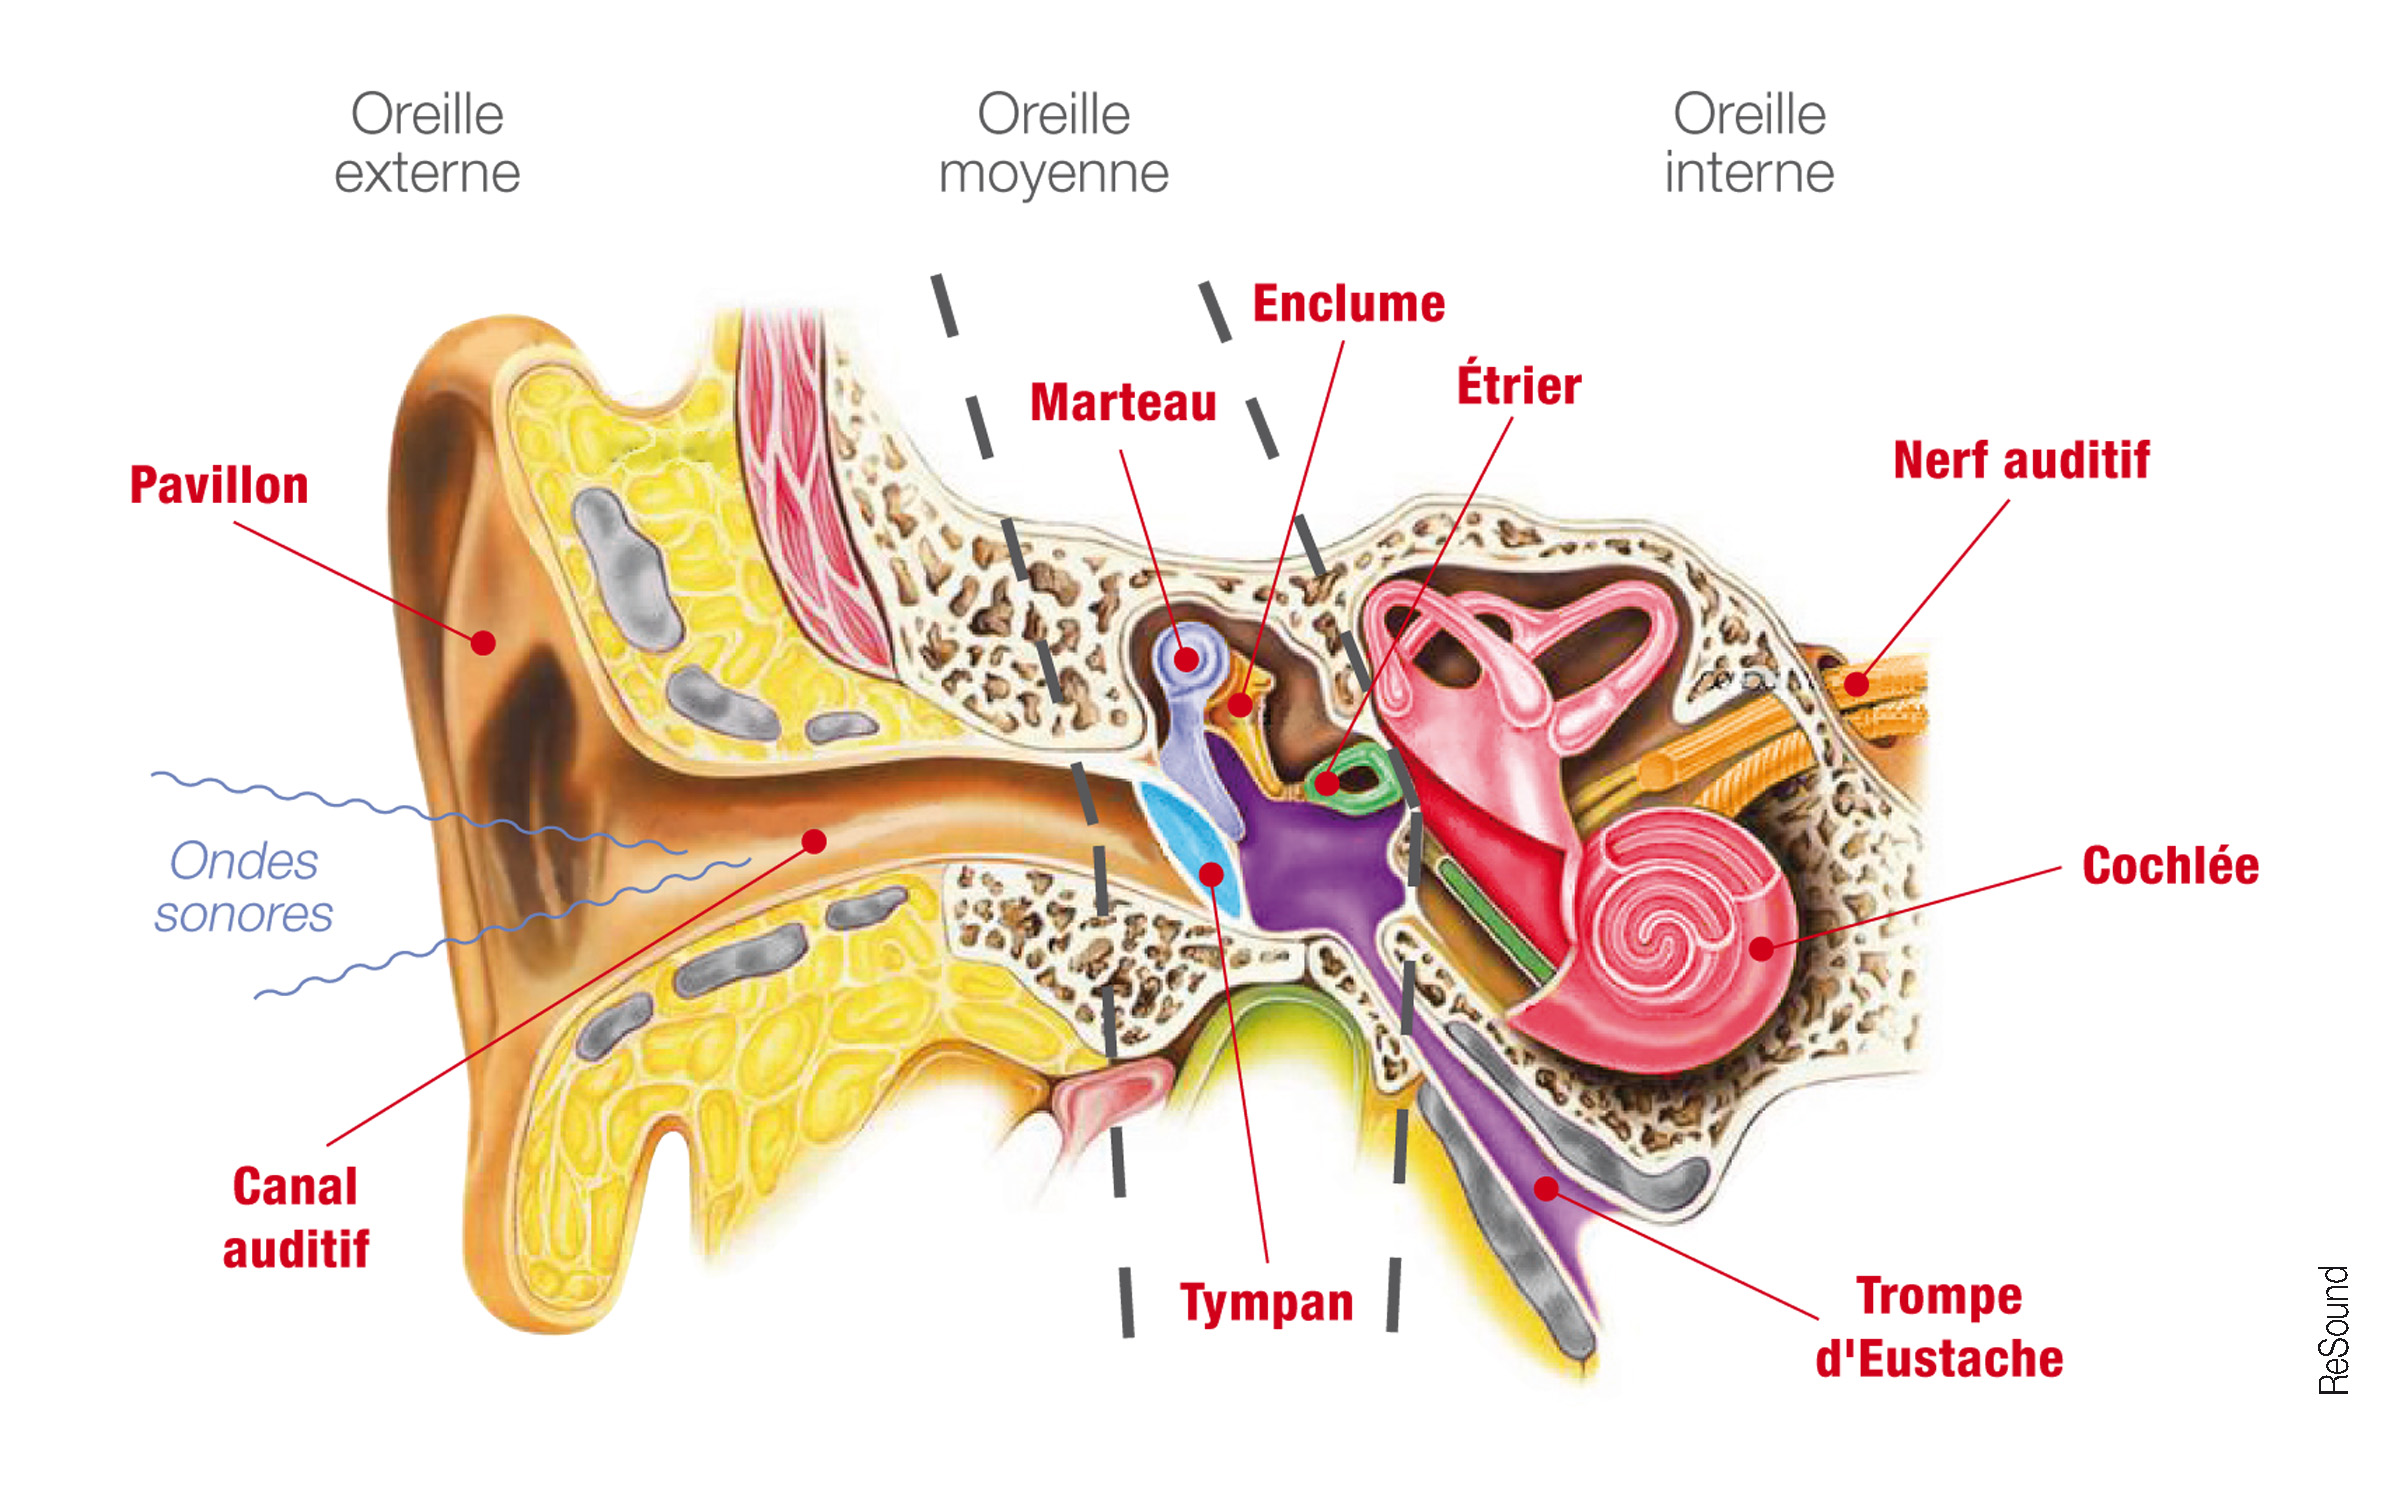
\includegraphics[width=0.8\textwidth]{../../../../Pictures/OREILLE.jpg}
% \caption[width=0.5\textwidth]{Schéma de l'oreille interne (http://www.mon-audition.info/wp-content/uploads/2015/01/OREILLE.jpg)}
% \label{fig:schemaOreille}
%\end{figure}
  
L'oreille humaine est composé de trois parties ayant chacune leur fonction : l'oreille externe  qui permet la localisation des sources, l'oreille moyenne qui joue le rôle d'amplification du son et l'oreille interne qui traduit la pression acoustique du signal en un signal électrique interpréter par le cerveau. Si le tympan et les osselets jouent le rôle d'adaptateur d'impédance entre l'extérieur et l'oreille interne, c'est la cochlée qui permet d'obtenir un signal électrique qui sera transmise au cerveau via le nerf auditif. \\

%\begin{figure}[hbtp]
% \centering
% 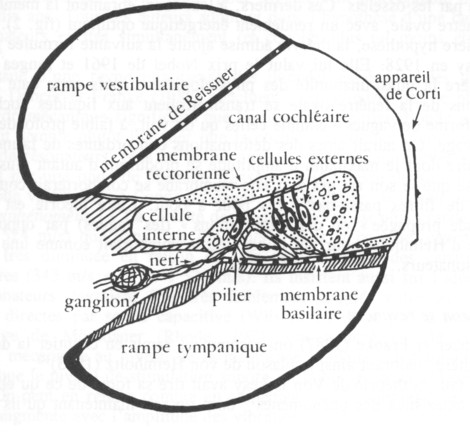
\includegraphics[width=0.4\textwidth]{../../../../Pictures/cochlea.jpg}
% \caption{Schéma en coupe d'une cochlée (http://auriol.free.fr/psychosonique/ClefDesSons/ecoute.htm)}
% \label{fig:schemaCochlé}
%\end{figure}

La cochlée consiste en une spirale creuse traversé par le canal cochléaire composé notamment de la membrane basilaire sur laquelle repose l'organe de Corti. Lorsqu'une onde acoustique arrive au tympan, elle est converti en énergie mécanique dont l'énergie est ensuite transmise à la cochlée grâce au osselets. Cette énergie met en mouvement la membrane basilaire à des positions localisées qui dépendent de la fréquence du signal. Par ce déplacement, les cellules cilié se trouvant dans l'organe de Corti vont alors bouger convertissant le signal mécanique en en signal électrique qui se propage ensuite jusqu'au cerveau à travers le nerf auditif (http://www.cochlea.eu/cochlee). C'est ensuite dans le cerveau que le son est interprété et que l'auditeur peut y mettre un sens. Pour cela, les évolution des caractéristiques acoustiques (niveau sonore, continuité temporelle et fréquentielle) du son aide à la compréhension et la distinction des sources présentes. \\

La CASA reprend donc ces éléments et cherche à traduire ces organes en étapes numériques, la première étant la modélisation de l'ensemble oreille externe/moyenne/interne.\\

\subsubsection{Analyse fréquentielle}

L'oreille externe et moyenne sont résumées en un simple filtre passe-haut. Ensuite, l'oreille interne est synthétisée par un filtrage cochléaire (cochléogramme). Ce filtre traduit la sélectivité fréquentielle de la membrane basilaire en la modélisant par une banque de filtres passe-bandes dans laquelle chaque filtre simule la réponse en fréquences d'un point particulier de la partition cochléaire. Les cellules ciliées étant les éléments dans la membrane qui transmettent les perturbations vers le nerf auditif, leur réaction est modélisée par un filtre de gammatone basé sur un filtre impulsionnel.\\

\begin{equation}
gt(t) = t^{n-1} e^{-2\pi bt } \cos(2\pi f_0 t+\phi)
\end{equation}

avec $t$, le temps en seconde, $n$, l'ordre du filtre, $f_0$, la fréquence centrale du filtre en Hz, $b$ la largeur de la bande passante en Hz et $\phi$ la phase (rad). En sortie de la cochlée, on préfère utilisé comme représentation temps-fréquence, un cochléogramme au spectrogramme qui permet de mieux mettre en évidence les basses fréquences grâce à une échelle logarithmique.\\

\subsubsection{Paramètre d'extraction}

Cette seconde étape vise à extraire plusieurs paramètres qui seront utile à l'étape de groupement (partie \ref{sec:groupement}) : 

\paragraph{Pitch et périodicité}
L'objectif consiste à déterminer les fréquences fondamentales et les phénomènes récurrent à partir de l'auto-corrélations $a(t,f,\tau)$ pour chaque oreille (corrélogramme) et de l'inter-corrélation $c(t,f,\tau)$ entre les signaux des deux oreilles $h_L$ et $h_R$(corrélogramme-croisé). 

\begin{equation}\label{eq:CASA_FAC}
a(t,f,\tau) = \sum h(t-n,f)h(t-n-\tau,f)w(n), 
\end{equation}

\begin{equation}\label{eq:CASA_FAC}
c(t,f,\tau) = \sum h_L(t-n,f)h_R(t-n-\tau,f)w(n).
\end{equation}

La somme pour chaque fréquence permet alors de déterminer les fréquences fondamentales présentes

\begin{equation}
A(t,\tau) = \sum_f a(t,f,\tau),
\end{equation}
\begin{equation}
C(t,\tau) = \sum_f c(t,f,\tau).
\end{equation}

Si plusieurs sources sonores sont simultanées et présente des différentes fréquences fondamentales, il existe un moyen pour les déterminer \cite{DeCheveigne20006}.
\paragraph{Corrélation croisée des voix}
Comme les réponses des filtres gammatone se recouvrent, plusieurs bandes peuvent réagir à une même harmonique. La corrélation autour des fréquences voisines permet alors de mieux connaitre le phénomène. celle-ci se définit comme l'inter-correlation au fréquences voisines des auto-corrélation normalisées. 
\begin{equation}
k(t,f) = \frac{1}{M}\sum_{\tau=0}^{M-1}\hat{a}(t,f,\tau) \hat{a}(t,f+1,\tau)
\end{equation}
\paragraph{Variation de l'intensité}
L'apparition ou la disparition de sources sonores pouvant d'accompagner d'une variation du niveau sonore. Des valeurs seuils sont déterminées pour détecter ces variations à partir de la dérivée de l'enveloppe du signal.

\paragraph{Modulation d'amplitude}
L'extraction des modulation d'amplitude des enveloppes permet de revenir à l'enveloppe du signal même. Une des méthodes couramment employé est l'utilisation des transformée de Hilbert ou bien l'amplitude absolue des signaux en sortie des filtres complexes de gammatone.

\paragraph{Modulation de fréquence}
Ce paramètre permet de rendre compte des régimes transitoires.  Deux techniques existent, la première méthode consiste revient à extraire les contours spatiales du cochléogramme, la seconde implique de calculer la réponse fréquentielle instantanée des signaux en sortie des filtres passe-bandes. 

\subsubsection{Représentation à niveau moyen}
Cette étape consiste à établir une représentation des paramètres précédents le plus souvent par segmentation. 
\subsubsection{Groupement des sources}\label{sec:groupement}

\subsubsection{Re-synthétisation}



La cartographie du signal permet ensuite de retrouver le signal perçu par l'auditeur. Elle se base sur des fonctions de corrélations (corrélogramme) visant à synthétiser les phénomènes de masquage et à faire ressortir les pics principaux des signaux
Enfin un second corrélogramme entre les signaux issus des deux microphones (simulant les deux oreilles) permettent la localisation des sources grâce à leur déphasage. La séparation des différentes sources se fait lors du cochléogramme à partir d'un masque binaire. Ce masque est généré par le spectrogramme de la source ciblé seul  puis pondère chaque trame \og temps-fréquence \fg{} du cochléogramme afin de ne conserver que la source souhaitée.\\

C'est donc une approche \textit{bottom-up} où d'un signal complexe on détermine l'ensemble des sources présentes.  Cette méthode est le plus souvent utilisée pour la séparation de signaux de paroles ou de musique \cite{BrownCASASpeech}, c'est-à-dire d'un signal harmonique et n'est donc pas adaptée pour celle de sons environnementaux plus complexes où la présence de contenus harmoniques est quasi inexistante. C'est donc une méthode très peu employée pour ces ambiances sonores.

\subsection{Les méthodes par dictionnaires}

\subsubsection{Analyse en Composantes Indépendantes}\label{part:ACI}

L'Analyse en Composantes Indépendantes (ACI) \cite{Herault} \cite{Comon} est une méthode appartenant aux méthode dite \textit{séparation de sources en aveugles}, c'est-à-dire qui sépare un ensemble de sources sonore d'une mixture sans (ou avec peu) informations sur celles-ci. Le plus souvent, cela équivaut à résoudre un problème sous déterminé. Le principe de la méthode consiste, à partir d'un réseau de capteurs, à trouver les sources présentes dans un signal audio en supposant leur indépendances les unes des autres. \\

L'illustration la plus couramment citée pour cette méthode est l'effet \og cocktail party \fg{} \cite{Cherry}. Cet effet résume la capacité de l'être humain à séparer la voix de l'interlocuteur avec qui il discute d'un flux sonore environnant bruyant composé d'autre discussions. Cette habilité est notamment permise par l'indépendance entre le signal \textit{voix} et le bruit ainsi que par l'écoute binaural du sujet. \\

L'ACI consiste alors à décrire les signaux de chaque capteur $x_n$ comme une combinaison linéaires des sources $s_n$ présentes, supposées indépendantes et pondérées par des effets propagatifs $a_{nn}$. Dans le cas du \og cocktail party \fg{}, on considère deux signaux (la voix et le bruit) où les capteurs sont les deux oreilles de l'auditeur. 

\begin{subequations}\label{eq:ACI1}
\begin{align}
x_1 &= a_{11} s_1 + a_{12} s_2 + \dots + a_{1N} s_N\\
x_2 &= a_{12} s_1 + a_{22} s_2 + \dots + a_{sN} s_N\\
x_n &= a_{n1} s_1 + a_{n2} s_2 + \dots + a_{nN} s_N
\end{align}
\end{subequations}

Le système \ref{eq:ACI1} est alors généralisé à un ensemble $N$ de sources par l'équation~(\ref{eq:ACI2}).

\begin{equation}\label{eq:ACI2}
\mathbf{x} = \mathbf{As}
\end{equation}

où $\mathbf{x}$ est de dimension $P \times 1$ comprenant l'ensemble des mesures réalisées par les capteurs, $\mathbf{s}$, de dimension $N \times 1$, résume les différentes sources présentes et $\mathbf{A}$, de dimension $P \times N$, une matrice déterministe résumant les aspects de propagation entre les sources et les capteurs. Cet aspect peut se révéler très intéressant lorsque les milieux dans lesquels évoluent les signaux sont complexes. Toutefois, l'estimation de la matrice $\mathbf{s}$ ne peut se faire que si le nombre de capteurs est égale ou supérieur aux nombres de sources présentes ($P \geq N$).\\

Le problème à résoudre devient alors

\begin{equation}
\text{min } I(\mathbf{A}^{-1}\mathbf{x})
\end{equation}

où $I(\mathbf{y})$ est une mesure de dépendance des coordonnées de la matrice $y$. Sa minimisation assure la meilleure indépendance possible des solutions du problème.
Il y a indépendance entre les sources lorsque 
\begin{equation}
p(\mathbf{x}) = \prod_{i = 1}^N p(x_i).
\end{equation}
où $p(\mathbf{x})$ est une fonction de densité de probabilité de $\mathbf{x}$. La mesure d'indépendance est ensuite déterminée par le calcul de la divergence de Kullback-Leibler que Comon \cite{Comon} a choisi en raison de ces propriétés.

\begin{equation}\label{eq:divKLICA}
D(\mathbf{y}) = \int p(\mathbf{y})\log\frac{p(\mathbf{y})}{\prod_{i = 1}^N p(y_i)} d\mathbf{y}.
\end{equation}

La minimisation de (\ref{eq:divKLICA}) rend alors les composantes moins dépendantes les unes des autres. Toutefois, il n'existe pas d'algorithme générique qui permettrait de résoudre le problème facilement \cite{CichockiICA}, des connaissances \textit{a priori} sur les sources ou sur l'environnement sont nécessaires pour exprimer au mieux l'indépendance comme l'évolution temporelle ou spatiale des signaux.  \\

L'application de cette méthode est prévue pour l'analyse et la compression de données, la détection bayesienne, la localisation de sources et enfin l'identification et la déconvolution de signaux en aveugles.\\

Si la technique peut sembler intéressante elle présente l'inconvénient de nécessiter un nombre de capteur égal ou supérieur au nombre de sources présentes. Dans un espace clôt, cette condition est supportable mais, dans le cadre urbain où le nombre de sources est important, cette contrainte rend son utilisation peu envisageable.\\

Les méthodes de séparation couramment utilisées ne sont donc pas des méthodes bien adapté à notre situation et ne peuvent donc pas être utilisé. Néanmoins, une autre technique appartement à la méthode de \textit{BSS} offre des résultats intéressant et prometteur et peut être envisagée pour des ambiances sonores urbaines : la Factorisation en Matrice Non-Négative.

%\subsection{Applications}
%
%L'utilisation de ces techniques dans le domaine de la classification et de la détection se fait couramment et dans des domaines diverses (
%
%Rappeler les applications diverses dans les images, le milieu médicale, textuelles.
%Dans le cadre des signaux audiophoniques :
%séparation des sources sonores afin de réaliser des commandes vocales, de restaurer des signaux audio indépendamment 
%paroles, musiques, sons environnementaux...
%
%Dans le cadre de la restauration audio, classifier par genres musicaux, artistes..., traitement actif du son également, reconnaissance ou commande vocale.
%Les sons environnementaux sont constitués des sons qui ne sont ni musicaux ni de la paroles. On trouve dedans les sons produits par l'Homme (bruit mécaniques) ou ceux produit par les animaux (bio-acoustique). Ce choix de distinctions provient de la nature des sons qui est beaucoup plus harmonique dans la parole et la musique que dans l'environnement.\\
%
%Dans le cadre des sons urbains, on trouve des études portant sur la reconnaissance des sons présents en ville (Defréville, Couvreur)

%\bibliographystyle{unsrt}
%\bibliography{../bibliographie}

%\end{document}